\documentclass[a4paper,10pt]{scrbook}

\usepackage{geometry}
\geometry{verbose,a4paper,tmargin=2.5cm,bmargin=2.5cm,lmargin=2.5cm,rmargin=2cm}

%
%  TURN THIS TO FALSE FOR THE FINAL VERSION
%
%
\newif\ifshowtasks\showtaskstrue


\usepackage[pdftex]{graphicx}

%\usepackage{ifthen}



% Macht beim fett schreiben auch das Mathe-Zeug fett
%
\newcommand{\allbf}[1]{\textbf{\boldmath#1\unboldmath}}

% FANCY CAPTION
% \caption[#1]{\textbf{#1}#1}
\newcommand{\mycaption}[2]{\caption[#1]{\textbf{\boldmath#1\unboldmath} #2}}







%%%
%%% Now you can use \ifcolor as follows
%%% \ifcolor
%%%    Text parsed by PDFLaTeX
%%% \else
%%%    Text parsed if PDFLaTeX is not used
%%% \fi
%%% 
\newif\ifcolor\colortrue



%
%   COLOR
%
%
\usepackage{color}
\definecolor{brightred}{rgb}{1,0.9,0.9}
\definecolor{brightgreen}{rgb}{0.9,1,0.9}
\definecolor{brightblue}{rgb}{0.9,0.9,1}
\definecolor{brightyellow}{rgb}{1,1,0.85}

\definecolor{lightred}{rgb}{1,0.75,0.75}
\definecolor{lightgreen}{rgb}{0.75,1,0.75}
\definecolor{lightblue}{rgb}{0.75,0.75,1}
\definecolor{lightyellow}{rgb}{1,1,0.75}

\definecolor{red}{rgb}{1,0,0}
\definecolor{green}{rgb}{0,1,0}
\definecolor{blue}{rgb}{0,0,1}

\definecolor{darkred}{rgb}{.7,0,0}
\definecolor{darkgreen}{rgb}{0,.7,0}
\definecolor{darkblue}{rgb}{0,0,.7}

\definecolor{white}{rgb}{1,1,1}
\definecolor{lightgray}{rgb}{0.95,0.95,0.95}
\definecolor{gray}{rgb}{0.5,0.5,0.5}
\definecolor{black}{rgb}{0,0,0}

\definecolor{marker}{rgb}{0.9,0.9,0.9}
\definecolor{urgent}{rgb}{1,0,0}
\definecolor{discreeturgent}{rgb}{1,0.5,0.5}
\definecolor{discreetcomment}{rgb}{0.25,0.9,0.25}
\definecolor{checked}{rgb}{0,.7,0}



%\newif\ifshowtasks\showtaskstrue
\newif\ifshowtasks\showtaskstrue
\newcommand{\task}[1]{\ifshowtasks\textcolor{discreeturgent}{~#1~}\else\fi}
\newcommand{\comment}[1]{\ifshowtasks\textcolor{discreetcomment}{~#1~}\else\fi}
\newcommand{\drain}[1]{}

%
%    LISTINGS
% \begin{lstlisting}[float,caption=A floating example]
%    for i:=maxint to 0 do
%    begin
%      { do nothing }
%    end;
%    Write(’Case insensitive ’);
%    WritE(’Pascal keywords.’);
% \end{lstlisting}
%
% for referencing line numbers use (*@\label{comment}@*)  inside the lstlistings enviroment
\usepackage{listings}
\ifcolor
          \lstset{							% general command to set parameter(s)
               escapeinside={(*@}{@*)},
               xrightmargin=0.5cm,					% for centering
               xleftmargin=1.5cm,					% .. \textwidth shrinks after the first time, which is stupid
               framexleftmargin=20pt,					% for having the numbers beneath the h rules
               framexrightmargin=0pt,
               framextopmargin=2ex,					% draw good looking space between the lines
               framexbottommargin=2ex,					%... and the listing
               frame=single,						% h rules top and bottom
               language=C,
               tabsize=4,
               numbers=left,
               numberstyle=\footnotesize, 
               numbersep=8pt,
               basicstyle=\ttfamily\scriptsize, 		% print whole listing small
               breaklines=true,
               keywordstyle=\color{black}\bfseries,		% underlined bold black keywords
               identifierstyle=,				% nothing happens
               commentstyle=\color{darkblue}\itshape,		% white comments
               stringstyle=\ttfamily, 				% typewriter type for strings
               morekeywords=[2]{and,or,not},
               emph={wichtiges,zeug},				% additional keywords
               emphstyle=\underbar,
               showstringspaces=false} 				% no special string spaces
\else
          \lstset{						% general command to set parameter(s)
               escapeinside={(*@}{@*)},
               xrightmargin=0.5cm,				% for centering
               xleftmargin=1.5cm,
               framexleftmargin=20pt,				% for having the numbers beneath the h rules
               framexrightmargin=0pt,
               framextopmargin=2ex,				% draw good looking space between the lines
               framexbottommargin=2ex,				%... and the listing
               frame=single,					% h rules top and bottom
               language=C,
               tabsize=4,
               numbers=left,
               numberstyle=\footnotesize, 
               numbersep=8pt,
               basicstyle=\scriptsize\ttfamily,			% print whole listing small
               breaklines=true,
               keywordstyle=\color{black}\bfseries,		% underlined bold black keywords
               identifierstyle=,									% nothing happens
               commentstyle=\color{black}\itshape,			% white comments
               stringstyle=\ttfamily, 							% typewriter type for strings
               morekeywords=[2]{and,or,not},
               emph={wichtiges,zeug},								% additional keywords
               emphstyle=\underbar,
               showstringspaces=false} 						% no special string spaces
\fi

%
\usepackage[labelfont={bf},font=small]{caption,subfig} 
% justification=raggedright,format=hang,labelfont={bf},font=small
% justification=justified,singlelinecheck=false

%
%    HYPERREF
%
%    (depends on z_layout_settings color)
%
% NO HANDLING YET FOR NOT PDF!!!
\ifcolor
  \usepackage[pdftex,
            colorlinks=true, linkcolor=blue, urlcolor=blue, citecolor=blue,
            raiselinks=true,
            bookmarks=false,
            bookmarksopenlevel=1,
            bookmarksopen=true,
            bookmarksnumbered=true,
            hyperindex=true,
            plainpages=false,% correct hyperlinks
            pdfpagelabels=true%,% view TeX pagenumber in PDF reader
            %pdfborder={0 0 0.5}
            ]{hyperref} % erzeuge Hyperlinks z.B. für pdflatex
\else
  \usepackage[pdftex,
            colorlinks=true, linkcolor=black, urlcolor=black, citecolor=black,
            raiselinks=true,
            bookmarks=false,
            bookmarksopenlevel=1,
            bookmarksopen=true,
            bookmarksnumbered=true,
            hyperindex=true,
            plainpages=false,% correct hyperlinks
            pdfpagelabels=true%,% view TeX pagenumber in PDF reader
            %pdfborder={0 0 0.5}
            ]{hyperref} % erzeuge Hyperlinks z.B. für pdflatex
\fi





\newcommand{\lstsetCPP}{%
\ifcolor%
\lstset{
	escapeinside={//(@*}{*@)},
	language=C++,
	frame=single,
	numbers=left,
	backgroundcolor=\color{brightblue}
	}%
\else%
\lstset{
	escapeinside={//(@*}{*@)},
	language=C++,
	frame=single,
	numbers=none,
	backgroundcolor=\color{white}
	}%
\fi%
}

\newcommand{\lstsetARCHEDXML}{%
\lstset{
	escapeinside={<!--(@*}{*@)-->},
	language=XML,
	frame=single,
	numbers=left,
	backgroundcolor=\color{lightyellow}
	}%
}

\newcommand{\lstsetJUSTXML}{%
\lstset{
	escapeinside={<!--(@*}{*@)-->},  % <!--(*@\label{comment}@*)-->
	language=XML,
	frame=single,
	numbers=left,
	backgroundcolor=\color{brightyellow}
	}%
}


\newcommand{\lstsetKSH}{%
\lstset{
	escapeinside={(@*}{*@)},
	language=ksh,
	frame=single,
	numbers=none,
	backgroundcolor=\color{lightgray}
	}%
}

% Sometimes latex just won't accept a line break.
% With this command you can do it anyway! HAR HAR HAR
\newcommand{\forcelinebreak}{
%\vspace{\bigskipamount}
\hspace*{\fill} \\
} 


\usepackage{framed}                                %for shaded and framed paragraphs
\usepackage{textcomp}                              %for various symbols, e.g. Registered Mark
%
\def\efill{\hfill\nopagebreak}%
\hyphenation{Nordu-Grid}
\setlength{\parindent}{0cm}
\setlength{\FrameRule}{1pt}
\setlength{\FrameSep}{8pt}
\addtolength{\parskip}{5pt}
\renewcommand{\thefootnote}{\fnsymbol{footnote}}
\renewcommand{\arraystretch}{1.3}
\newcommand{\dothis}{\colorbox{shadecolor}}
\newcommand{\globus}{Globus Toolkit\textsuperscript{\textregistered}~2~}
\newcommand{\GT}{Globus Toolkit\textsuperscript{\textregistered}}
\newcommand{\ngdl}{\url{http://ftp.nordugrid.org/download}~}
\definecolor{shadecolor}{rgb}{1,1,0.6}
\definecolor{salmon}{rgb}{1,0.9,1}
\definecolor{bordeaux}{rgb}{0.75,0.,0.}
\definecolor{cyan}{rgb}{0,1,1}
%
%----- DON'T CHANGE HEADER MATTER

\hypersetup{
  pdfauthor = {},
  pdftitle = {Webservices},
  pdfsubject = {Paper subject},
  pdfkeywords = {HED,ARC},
  pdfcreator = {PDFLaTeX with hyperref package},
  pdfproducer = {PDFLaTeX}
}

\begin{document}


% BASIC CONCEPT

% * Installation

% * Usage

% * Maintainance

% * Programming concept
 
% * Future work

% * APPENDIX


 \def\today{\number\day/\number\month/\number\year}

\begin{titlepage}

\begin{tabular}{rl}
\resizebox*{3cm}{!}{
\includegraphics{images/ng-logo.png}}
&\parbox[b]{2cm}{\textbf \it {\hspace*{-1.5cm}NORDUGRID\vspace*{0.5cm}}}
\end{tabular}

\hrulefill

{\raggedleft NORDUGRID-TECH-19\par}

{\raggedleft \today\par}

\vspace*{2cm}

%%%%---- The title ----
{\centering \textsc{\Large Webservice programming Tutorial}
\\\vspace{1cm} \normalsize\textcolor{discreeturgent}{I am currently working on this document, but I appreciate all comments and suggestions. \\e-mail: glodek@inb.uni-luebeck.de} % DELETE ONLY THAT LINE!!!
\Large \par}
\vspace*{0.5cm}

%%%%---- A subtitle, if necessary ----
%{\centering \textit{\large Paper subtitle}\large \par}

\vspace*{1.5cm}
%%%%---- A list of authors ----
    {\centering \large Michael Glodek, Steffen M\"oller, ... \large \par}

%%%%---- An abstract - if style is article ----
%\begin{abstract}
%The abstract
%\end{abstract}
\end{titlepage}

\tableofcontents                          %Comment if use article style
\newpage
%\chapter{Preface}
%\section{Introduction}                    %Use Sections for articles
%\label{sec:intro}

\sloppy


\chapter{Introduction}

This document gently introduces to the preparation of standalone Web Services and cognated clients with the Advance Resource Connector (ARC).
The reader is guided through a series of practically oriented examples.
Each is accompanied by explanations of the main concepts of the software architecture.
No particular skills are required to follow the presented steps.
It is however beneficial to have some basic comprehension of the programming language C++, the file format XML and any regular UNIX shell.
To start, the user shall have an installation of ARC-1, as it is performed with current RPM or .deb packages\footnote{see http://wiki.nordugrid.org for explicit instructions for setup}.\\


The ARC server provides access to services.
These are executed on the same machine that the server is installed on.
Some services, like the A-REX service, will delegate computational efforts to other machines
via additional software like a local queueing system.
But the A-REX service itself does not migrate away to other machines - at least this
has not been implemented yet.
Services may comprise computational tasks (e.g., some secret and strongly
patented algorithm), allow arbitrary computations (like ARC's A-REX or
Amazon's clouds) or provide access to other resources like a particular
database or to arbitrary disk space (like ARC's hopi or bartender).\\


Services are invoked using software programs, which are referred to as clients. 
These programs may directly perform the interactions of human users or request a performance of other services of another server (here the first service is in the role of a client, too).
The tasks of servers and clients are well defined. If servers are not busy reacting to a client's request, then they are waiting. The task of servers can be subdivided into:
\begin{itemize}
 \item Wait for client request
 \item Receive the request
 \item Perform the desired service
 \item Create a response for the client
 \item Send response to the client
 \item Wait for next client request
\end{itemize}
While the server waits passively for a request, the client acts actively:
\begin{itemize}
 \item Create a request
 \item Transmit the request to the server which provides the desired service.
 \item Wait for the reply
 \item Receive the response from the server.
 \end{itemize}
Servers provide access to a single or a set of services. In ARC services are provided by the Hosting Environment Demon (HED) which enables the installation of several services on one network access point. 
\forcelinebreak

In general, the implementation of a client is easier than the implementation of the server. 
ARC is designed as a middleware which encapsulates typical challenges of server-client infrastructures (security, exception handling, extensibility) and abstracts from the underlying computer architecture (heterogeneity of computers, computer location, protocols).
The core of ARC is the prior mentioned HED (Hosting Environment Daemon).
To the administrator HED is mostly visible as the single binary that is started and configured by a file that describes services' that shall be prepared by HED. 
Conceptionally, the HED determines how services shall be organised both as a principle, and for any given ARC-run server.
HED determines the very explicit presence or absence of a service at a particular address. Its many configurable layers are described later in this tutorial. 
%
At the time of writing, the endpoint of the HED will be a SOAP based  Web Service.
SOAP is a long established XML-based standard for Web Service communication.
ARC abstracts from this format, but nevertheless it is useful to be aware of
the underlying message transport mechanism.

%which implicate several advantages.
%The XML file format is not restricted to a certain set of tags but can be expanded in such a way as to fit almost any kind of service. It is not a proprietary format and as a result many libraries in almost any language are capable in creating that kind of format.Likewise, XML is also suitable for the usage between heterogeneous platforms.However, while the client can be implemented very straight, the service has to fit a certain layout.In the present guide four kinds of webservices will be introduced: a simple time service, an echo service, a secure echo service and a service with a persistence state .\\


 


\section{Hosting Environment Daemon}

The HED which was already mentioned in the section above is an essential part of the ARC middleware. 
Its task is to provide the hosting of various services at the application level and is based on the idea modularity. % allows its dynamic extension.
The HED consists of components called Message Chain Components (MCC), Plexer, Services, and several modules, which shall aid the programmer to simplify the development of the Web Services: Config, Loader, Logging, XMLNode et cetera.
The MCCs are ordered within a layered structure. 
Each MCC provides a certain functionality such as communication between two applications (MCC TCP), secure data transfer (MCC TLS) or client-server architecture (MCC HTTP).
Figure~\ref{fig:HED_internal} illustrates a typical setup of a server-sided HED.

\begin{figure}[htb]
	\centering
	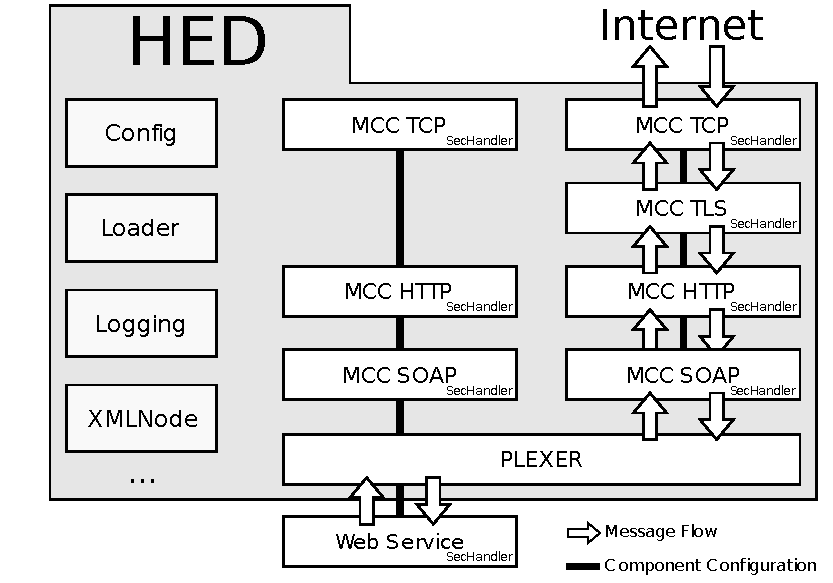
\includegraphics[width=13cm]{tex_introduction/HED2.pdf}
	\mycaption{Example of a HED structure providing a Web Service}{The HED consists of several layers which are connected with each other. The arrow indicate the message flow of the used configuration. The MCCs and Services may hold a SecHandler in order to give additional security. Additional modules (on the left) are used within the HED. \task{Why is the Web Service in all images outside of the HED?} } % TODO: Reverse order of layers, s.t. the highest layers are above and the lowest layer are at the bottom
\label{fig:HED_internal}
\end{figure}

The MCCs are connected which each other and passing incoming and outgoing message to the upper or the respective lower layer. In case of outgoing messages a MCC is wrapping the data of the upper layer as a payload into their own protocol (while incomming message will be unwrapped).
The lowest layer has to be a transport protocol like TCP which enables the transmission between two applications.
Technically there are even lower layers required needed for the communication but they are already realised within the operating system and the  network card.
TCP is well suited for the application because it provides a reliable and ordered delivery of a byte stream.
Above the TCP layer is the Hypertext Transfer Protocol (HTTP). 
In case a security layer is desired (i.e. for authentication), the TLS (Transport Layer Security formerly known as SSL, Secure Sockets Layer) has to be inserted between the TCP and HTTP layers.
The HTTP provides the client-server architecture. It is stateless but offers several extensions for requests, header information and status codes. Furthermore HTTP enables the usage of Uniform Resource Locators (URL) which is used by ARC to multiplex between different services. The multiplexing layer can also be defined within the HED and is called Plexer.
Depending on the path of the URL the Plexer passes messages to a defined SOAP service which again passes the message to the Web Service~\cite{QIANG_2005}.\\
% QUESTION: Why is the plexer always illustrated  being above the SOAP MCC. There's no config file example like that in the tree.
%In my understanding (because plexer is not my initial idea), plexer (as a sort of hub) can be put at both after http or soap. If you put after soap,then you are doing switching for different web services. While I put it after http, because somehow, I need to switch the message after http-processing, in more detail, one branch for soap and then web service/s, one branch for a non-soap service/server (the SP Service is not a service based on SOAP, actually it is based on http, so it is kind of web application).


The structure of the HED can be configured freely by modifying the server configuration file.
A first impression how the HED can be configured shall be given in the following example which corresponds to the HED shown in Figure~\ref{fig:HED_internal}.
It uses the ARC echo service that is shipped for testing purposes with the ARC source code.



\subsection{The ARC Echo Web Service}
\label{sec:arc_echo_web_service}


The first example shall give a basic understanding in how to configure the HED for setting up a novel service.
The task is to setup the regular ARC Echo Web Service.
On the command line, all that needs to be done is to invoke the \textit{arched} daemon with a suitable server configuration file.
Such a fitting server configuration file is shown in Listing~\ref{lst:arched_arcecho_xml}.
It is written in XML. Its structure is based on the XSD schema listed in~\ref{sec:impXSD} in Listing~\ref{lst:mcc.xsd}.\\ 

\lstsetARCHEDXML
\lstinputlisting
	[label=lst:arched_arcecho_xml,float=htb,
	caption={[HED configuration file.]
	\textbf{HED configuration file.}}]
{../examples/src/services/arched_arcecho.xml}
The first line of the XML file contains the XML declaration.
Several attributes can be defined here but at least the XML version should be specified.
The configuration as a whole is encapsulated by the element \textit{ArcConfig}. It also performs the setting of namespaces, which are expected to be mostly invariant across all server installations. % ABBREVIATIONS?? - MG
The \textit{Server} element, to be found at line~\ref{lst_code:arched_arcecho_Server}, provides basic settings for the daemon such as the location of the Pid-file or ofthe Log-file.
The \textit{ModuleManager} holds the \textit{path} to the plugin libraries.
Several paths may be defined here.
Due to the fact that the first library matching the plugin name is loaded, the order is relevant.
The path should be at least assigned to the ARC installation directory.
Otherwise, the set of ARC MCC plugins might not be found.
The next elements are holding the name of the plugins to be loaded (line~\ref{lst_code:arched_arcecho_Plugins}).
The names have to correspond to the names of the dynamic libraries within the path defined in the \textit{ModuleManager}.
Finally, the chain, which creates the layered structure, is declared within the element \textit{Chain}.
It is composed of the elements \textit{Component}, \textit{Plexer} and \textit{Service}.
Due to a MCC plugin may contain several components, one has to specify more exact which one to load. This is to be done using the \textit{name} attribute i.e. the plugin \textit{mcchttp} realises two components: \textit{http.service} and \textit{http.client}. Since we are defining a configuration file for a service, the \textit{http.service} should be used.
Furthermore the elements may have the attribute \textit{id} as a unique identifier within the file.
Regarding the components and the services a plugin (implemented as a *.so file that is searched in the paths previously specified) has to be loaded which provides the implementation of its functionality. The further configuration depends on the plugin's individual functionality.\\
%
% within the chain ... 3 types of elements
%
%Its needed to distinguish between the plugins and the components.
%The plugins refer to shared libraries that can be integrated as modules with the HED to extend its functionality.
%The Components refer to the implementation of Web Services within any of those libraries.


A \textit{Chain} will determine the path that an event takes to be noticed.
The first component of the chain is the \textit{tcp.service}.
As to be seen, the port 60000 is assigned to the server to listen to.
The port can be an arbitrary number.
However, the number 60000 is commonly used for a HED providing the A-REX Web Service (the one organising the computation on a site) and the number 50000 is found commonly used for a HED running Web Services for storage.
This way, one can organise a single server to offer multiple HED instances.
The stream which is received by this component is passed to the component defined by the \textit{next} attribute.
In the present case, it will be passed to the component with the \textit{id} attribute named \textit{http}.
In this way, the message is be passed to higher layers until it reaches the \textit{Plexer}.
Depending on the path of the URL which was demanded by the HTTP, the Plexer multiplexes the request to the right Web Service\task{, the right function to execute according to the component IDs and plugin names. -- ??MG}
The plexer will thus allow to have multiple Web Service listen to the same port.
The path, declared within the \textit{next} attribute, corresponds to a regular expression and leads to the service with the id named \textit{echo}. 
Hence, the service will now be reachable under URL \textit{http://localhost:60000/echo}.
It will finally process the message and create a new message which will be returned all the way back to the TCP component.
The Echo Web Service itself is provided by the ARC package.
Additional invariant parameters are passed by the elements \textit{prefix} and \textit{suffix}.
They set the characters which will enclose the echoed string.
\task{The images of the HED structure always are ordered like: TCP - TLS - HTTP - PLEXER - SOAP - Web Service   but the source code examples are: TCP - TLS - HTTP - SOAP - PLEXER - Web Service}

To create the daemon corresponding to the defined server configuration file, ARC provides the program called \textit{arched}.
The manner of invokation is to been seen in Listing~\ref{lst:arcecho_arched_invokation}.
\lstsetKSH
\begin{lstlisting}[
label=lst:arcecho_arched_invokation,float=htb,
caption={[Invokation of the arched daemon in order to start the ARC Echo Web Service.]
         \textbf{Invokation of the Arched Daemon.\textcolor{white}{hmf}}}]

$ arched -c arcecho_no_ssl.xml && echo Daemon started || echo Daemon failed
 Daemon started
$
\end{lstlisting}

% $ rm -f /var/log/arched.log
% $ tail -n100 -f /var/log/arched.log
%...
%$ killall arched
%
%
The name of the program is followed by the parameter \textit{-c}.
The string following that argument contains the path to the configuration file.
Once the server is running, the client can be used as described in Listing~\ref{lst:arcecho_client_invokation}.
\lstsetKSH
\begin{lstlisting}[
label=lst:arcecho_client_invokation,float=htb,
caption={[Usage of the ARC Echo client.]
         \textbf{Usage of the Arc echo client.\textcolor{white}{hmf}}}]
$ arcecho http://localhost:60000/Echo text
[ text ]
\end{lstlisting}

In this example, the server and the client are running on the same computer such that the hostname \textit{localhost} can be utilized. 
For debugging it is advisable to check the logfile which was assigned inside the server configuration file.
It is commonly found at /var/log/arched.log.

The following chapters explain how to develop custom Web Services.
The first one will be the simple Time Web Service.












 % 1 
\chapter{Installation} 


% ** Dependencies
% *** Ordinary: log4perl and ``Redland RDF Library - Perl Interface''
% *** WebService: libperl-dev
% *** Protege: For maintaining the knowledge base


The Janitor requires the two perl packages listed in
table~\ref{tab:installDependencies}. To have the WebService
interface for the Janitor, the packages listed in
table~\ref{tab:installDependenciesOptional}
need to be installed before
the build process is. The Perl modules are available on CPAN and ship
with all major Linux distributions.  

\begin{table}[!h]
   \begin{center}
        \mycaption{Required perl packages for the Janitor.}
		   {Log4perl is used for the internal logging of the
		   Janitor, while the Redland RDF library is used
		   for accessing the knowledge base (catalog) of
		   Runtime Environments.}
        \label{tab:installDependencies}
	\begin{tabular}{|p{3cm}|p{7cm}|}
	\hline
	   liblog-log4perl-perl & \textit{Log4perl is a port of the log4j logging package}\\
	\hline
	   librdf-perl          & \textit{Perl language bindings for the Redland RDF library}\\
	\hline
	\end{tabular} 
   \end{center}
\end{table}
\begin{table}[!h]
   \begin{center}
        \mycaption{Optional libraries for the Janitor.}{The
		   library libperl-dev provides the required header files to link the 
                   WebService to the Perl interpreter.}
        \label{tab:installDependenciesOptional}
	\begin{tabular}{|p{3cm}|p{7cm}|}
	\hline
	   libperl-dev & \textit{ Perl library: development files}\\
	\hline
	\end{tabular}
   \end{center}
\end{table}
\forcelinebreak

If you are using regular Debian or Ubuntu packages, then the Janitor
can be installed as root by "apt-get install nordugrid-arc1-janitor".
Installing it will not drag other components of ARC with it, since the
Janitor can be used in its own right -- or in conjunction with another
grid system, possibly. Packages for Redhat/Fedora and SuSE/OpenSuSE are
also provided, the redland library however may not yet be available for
those systems.

The Janitor source code is shipped as a part of the regular ARC-NOX
source tree.  If you are compiling the sources yourself, the default
is to have the A-REX grid manager technically prepared to interact
with the Janitor.
The interaction can be prohibited
with the \textit{configure} flags \textit{--disable-janitor-service}
for the complete janitor or \textit{--disable-janitor-webservice} for
only the Web Service support.

Furthermore many users will want to consider installing the ontology editor 
Prot\`eg\`e\footnote{\href{http://protege.stanford.edu}{http://protege.stanford.edu}}
to easily maintain the knowledge database of installable
packages.  At the time of writing, no Linux distribution is offering
packages for this fine tool. However, the basic editing can also be
performed fairly easily without that tool, and everyone is working on
simplifying that process.


\section{Configuration}\label{sec:janitorConfiguration}

The current version of the Janitor can be configured using the
common file \textit{arc.conf}. It is expected in the configuration
directory \textit{etc}. The Janitor is using the environment
variable \textit{NORDUGRID\_CONFIG} to determine the location of the
corresponding file. If that variable is not set, the default location
\textit{/etc/arc.conf} will be used.  The configuration is assigned
by the section \lbrack janitor\rbrack. Table~\ref{tab:arcConfTags}
describes the available tags for the Janitor's configuration.

\begin{landscape}
\begin{table}[!h]
   \begin{center}
        \mycaption{Tags usable in \textit{arc.conf} within the section janitor.}{Tags usable in \textit{arc.conf} within the section janitor.}
	\label{tab:arcConfTags}
	\begin{longtable}{|p{3cm}|p{10cm}||p{10cm}|}
	\hline
	   \textbf{tag}    & \textbf{example}                      & \textbf{description}\\
        \hline
           enabled         & "1"                                   & Boolean flag which enables or disables janitor in A-REX.\\
	   uid             & "root"                                & The effective uid. \\
	   gid             & "0"                                   & The effective gid. \\
	   registrationdir & "/var/spool/nordugrid/janitor"        & Directory where we the current states of jobs are kept. \\
	   catalog         & "/var/spool/nordugrid/janitor/catalog/knowarc.rdf"& URL of the catalog containing the package information.\\
	   downloaddir     & "/var/spool/nordugrid/janitor/download" & Directory for downloads \\
	   installationdir & "/var/spool/nordugrid/janitor/runtime"& Directory for installation of packages                   \\
	   jobexpirytime   & "7200"                                & If a job is older than this, it is considered dead and assigned to be removal pending.\\
	   rteexpirytime   & "36"                                  & If a runtime environment was not used for this time, it will be assigned to be removal pending.\\
	   allow\_base     & "*"                                   & Allow rule for base packages. \\
	   deny\_base      & "debian::etch"                        & Deny rule for base packages.\\
	   allow\_rte      & "*"                                   & Allow rule for base packages. \\
	   deny\_rte       & "APPS/MATH/ELMER-5.0.2"               & Deny rule for base packages. \\
	   logconf         & "/opt/nordugrid/etc/log.conf"         & Location of the logging configuration file for janitor.\\
	\hline
	\end{longtable}
   \end{center}
\end{table}
\end{landscape}

The parameter \texttt{enabled} specifies whether the Janitor shall be used
within A-REX or not. This needs to be distinguished from the previously mentioned
compilation flags of a similar name. Use the value \texttt{"0"} to disable Janitor. The
\texttt{uid} and the \texttt{gid} are defining which effective user id
(uid) and group id (gid) shall be used for the Janitor.

The \texttt{registrationdir} describes the directory in which the
subdirectories \texttt{jobs} and \texttt{rtes} will be created.
In these directories the states of the jobs and the runtime environments
are stored. Please recall that the Janitor does not use a database as
a backend, but all communication between invocations are performed via
files in those folders.

The knowledge base of installable packages is specified by the parameter
\texttt{catalog}.  Its value can be any kind of URL pointing to a file
written in the Resource Description Framework (RDF) format.  One should
not light-heartedly use a remote address for this purpose. Such a remote
source needs to be trusted, since any runtime environment specified in
a catalog (if the package description matches constraints by the local
site administrator) may possibly be installed by regular grid users.

The specification of the RDF file will be explained in detail in
section~\ref{sec:catalog}.  The parameter \texttt{downloaddir} assigns
the directory to which the installation files will be saved after they
have been downloaded or copied from the repository which was specified by
the catalog. Please remember: the URL in arc.conf indicates the location
of the catalog. And the URLs somehow specified in the catalog specify
the location from where to download the runtime environment.

The \texttt{installationdir} finally specifies the directory into which
all packages will be installed. This directory needs to be available
for all computing nodes for the execution of arbitrary programs, most
commonly by using it as a shared NFS volume.

If the configuration file furthermore contains the \texttt{runtimedir}
tag within the section \texttt{grid-manager}, the Janitor will also
create a symbolic link in the \texttt{runtimedir} pointing to the
configuration script of the installation performed by the Janitor.
The tags \texttt{jobexpirytime} and \texttt{rteexpirytime} are used
for an automated cleanup and is defined in seconds.  The default
value for the \texttt{jobexpirytime} is seven days and for
the \texttt{rteexpirytime} three days.  The additional tags
\texttt{allow\_base} \texttt{deny\_base} \texttt{allow\_rte} and
\texttt{deny\_rte} are used to include or exclude certain base packages
or runtime environments of the catalog. This feature is useful, if the
catalog is maintained by a higher organization. But again: you need to
trust it.

The path to the log4perl configuration file is defined by the tag
\texttt{logconf}.  Examples on how to configure ARC and log4perl are
provided in the Listings~\ref{lst:arcConf} and ~\ref{lst:logConf}.


\lstsetCONFIGURE
\begin{lstlisting}[
        label=lst:arcConf,
        caption={ [Example \textit{arc.conf} settings for janitor.]
                  \textbf{Example \textit{arc.conf} settings for janitor.}}
        ]
[janitor]
enabled="1"
logconf="/opt/nordugrid/etc/log.conf"
registrationdir="/var/spool/nordugrid/janitor"
installationdir="/var/spool/nordugrid/janitor/runtime"
downloaddir="/var/spool/nordugrid/janitor/download"
jobexpirytime="7200"
rteexpirytime="36"
uid="root"
gid="0"
allow_base="*"
allow_rte="*"

[janitor/nordugrid]
catalog="/var/spool/nordugrid/janitor/catalog/knowarc.rdf"
\end{lstlisting}

It should be noted that the downloaddir or the installationdir specified
in arc.conf could be any directory. Those will not be prepared by the
package for the Linux distribution but need be created by the administrator
manually after the Janitor has been installed. This also holds for the
catalog.

When working with several catalogs, then the multiple catalog lines can
be placed into the same arc.conf file. But every must go into its own block
as separated with \[janitor/someName\] directives.

\lstsetCONFIGURE
\begin{lstlisting}[
        label=lst:logConf,
        caption={ [Example \textit{log.conf} settings for janitor.]
                  \textbf{Example \textit{log.conf} settings for janitor.}}
        ]
# Master Loglevel
# [OFF | DEBUG | INFO | WARN | ERROR | FATAL]
#log4perl.threshold = OFF

log4perl.rootLogger = WARN, DebugLog, MainLog, ErrorLog
log4perl.appender.DebugLog = Log::Log4perl::Appender::Screen
log4perl.appender.DebugLog.layout = PatternLayout
log4perl.appender.DebugLog.layout.ConversionPattern = [%C] %d %p> %m%n

log4perl.appender.MainLog = Log::Log4perl::Appender::File
log4perl.appender.MainLog.Threshold = DEBUG
log4perl.appender.MainLog.filename = /var/log/janitor.log
log4perl.appender.MainLog.layout = PatternLayout
log4perl.appender.MainLog.layout.ConversionPattern = %d %p> %m%n

log4perl.appender.ErrorLog = Log::Log4perl::Appender::File
log4perl.appender.ErrorLog.Threshold = ERROR
log4perl.appender.ErrorLog.filename = /var/log/janitor_error.log

log4perl.appender.ErrorLog.layout = PatternLayout
log4perl.appender.ErrorLog.layout.ConversionPattern = %d %p> %m%n
\end{lstlisting}


% ** Configuring arc.conf
% *** Where to store the data of janitor
% ** Configuring log.conf
% *** Where to store the log of janitor

\section{Limitations}

The Janitor was designed to be used for UNIX-compatible operating systems
and tested for various Linux distributions. It should also be functional
on MaxOS X and Windows with Cygwin or coLinux.  The porting of the Janitor
to other platforms has not yet been addressed.

The ARC middleware is not ultimately essential for dynamic Runtime
Environments.  All the Perl code would be functional with any Grid
middleware.

% 2
\chapter{Usage}

The Janitor can be used either with or without the A-REX service.
In case
A-REX is used, the invocation of the Janitor will be performed in an
automated manner.  It is then triggered by incoming jobs that request
a particular RTE for their execution.  If it is not already installed,
but
\begin{enumerate}
\item found as a MetaPackage in a Catalog that the site supports
\item with a package that first the BaseSystem of the site
\end{enumerate}
then it will be installed without further manual intervention by the
Janitor - triggered by the A-REX that received the compute request.

The Janitor's installation will not be affected by this decision
pro or cons and integration with \AREX. Both can be installed in
parallel. If \AREX is not allowed to install runtime environments upon
demand, such automated installations can still be invoked manually via
the Janitor's command line  interface.

\section{Janitor with A-REX}

Runtime Environments can be specified using the supported job description
languages.  The most representative two common languages shall be
explained at this point: xRSL and JSDL.  Listing~\ref{lst:xrsl_job}
shows the xRSL example in which two runtime environments are requested.

\lstsetXRSL
\begin{lstlisting}[
        label=lst:xrsl_job,
        caption={ [Job submission using the xRSL job description language.]
                  \textbf{Job submission using the xRSL job description language.}}
        ]
 &
 (executable = "run.sh" )
 (arguments = "weka.classifiers.trees.J48" "-t" "weather.arff")
 ("inputfiles" = ("weather.arff" "" ))
 ("stderr" = "stderr" )
 ("stdout" = "stdout" )
 ("gmlog" = "gmlog" )
 ("runtimeenvironment" = "APPS/BIO/WEKA-3.4.10")
 ("runtimeenvironment" = "APPS/BIO/WISE-2.4.1-5")
\end{lstlisting}
\task{The runtime environment names are composed out a directory name, the package name and the version number.}

A comprehensive reference manual of the Extended
Resource Specification Language (XRSL) can be found at
\href{www.nordugrid.org/documents/xrsl.pdf}{www.nordugrid.org/documents/xrsl.pdf}~\cite{NORDUGRID_MANUAL_4}.
Within Listing~\ref{lst:jsdl_job} an example using JSDL is provided. The
specification of how to assign runtime environments in JSDL is currently
only defined within the nordugrid jsdl-arc schema~
\href{http://svn.nordugrid.org/repos/nordugrid/arc1/trunk/src/services/a-rex/grid-manager/jobdesc/jsdl/jsdl_arc.xsd}
     {http://svn.nordugrid.org/repos/nordugrid/arc1/trunk/src/services/a-rex/grid-manager/jobdesc/jsdl/jsdl\_arc.xsd}.
\lstsetJUSTXML
\begin{lstlisting}[
        label=lst:jsdl_job,
        caption={ [Job submission using JSDL.]
                  \textbf{Job submission using JSDL.}}
        ]
<?xml version="1.0" encoding="UTF-8"?>
<JobDefinition
  xmlns="http://schemas.ggf.org/jsdl/2005/11/jsdl"
  xmlns:posix="http://schemas.ggf.org/jsdl/2005/11/jsdl-posix"
  xmlns:arc="http://www.nordugrid.org/ws/schemas/jsdl-arc">
  <JobDescription>
    <Application>
      <posix:POSIXApplication>
        <posix:Executable>/bin/sleep</posix:Executable>
        <posix:Argument>120</posix:Argument>
      </posix:POSIXApplication>
    </Application>
    <DataStaging>
      <FileName>test.sh</FileName>
      <Source/>
      <Target/>
    </DataStaging>
    <DataStaging>
      <FileName>transferGSI-small</FileName>
      <Source>
        <URI>gsiftp://pgs02.grid.upjs.sk:2811/unixacl/transferGSI-small</URI>
      </Source>
      <Target/>
    </DataStaging>
    <Resources>
      <arc:RunTimeEnvironment>
        <arc:Name>APPS/BIO/WISE-2.4.1-5</arc:Name>
        <arc:Version><Exact>2.4.1</Exact></arc:Version>
      </arc:RunTimeEnvironment>
      <arc:RunTimeEnvironment>
        <arc:Name>APPS/BIO/APPS/BIO/WEKA-3.4.10</arc:Name>
        <arc:Version><Exact>3.4</Exact></arc:Version>
      </arc:RunTimeEnvironment>
    </Resources>
  </JobDescription>
</JobDefinition>
\end{lstlisting}


\section{Janitor without A-REX}

On Linux systems, the Janitor's standalone commandline tool is
available as /usr/lib/arc/janitor.  Some Linux distributions may
prefer /usr/libexec or similar paths.  The script is only functional as
root\footnote{Should you find that constraint unbearable for your purpose,
please investigate the file rjanitor.cc in the ARC source tree. It wraps
the janitor application and as a C binary can be configured to attract
root privileges.}.  To find that binary directly, you may decide to add
that location to your \$PATH environment variable.

The available commands to the Janitor, implemented as options to the janitor script, are listed
in the Table~\ref{tab:janitor_commandline_man}.

\begin{table}[!h]
   \begin{center}
        \mycaption{Overview about the available commands to the Janitor.}{}
        \label{tab:janitor_commandline_man}
	\begin{tabular}{p{0.5cm}p{2cm}p{11cm}}
	\multicolumn{3}{l}{\textbf{janitor [COMMAND] [JOB-ID] [RTE] \dots}} \\
	\multicolumn{3}{l}{\textbf{Command:}}\\
	&	register & Registers a job and a set of runtime
			   environments in the Janitor database.
			   Requires the parameters [JOB-ID] and a list of [RTE]s.\\
	&	deploy	 & Downloads and installs the desired
			   runtime environments. Requires the name
			   of an already registered [JOB-ID].\\
	&	remove	 & Removes the placeholder of the job on the runtime environments.
			   If no more jobs are using the runtime environment and the
			   lifespan of the runtime environment has be expired, the runtime
			   environment can be removed using the \texttt{sweep} command.
			   Requires the [JOB-ID] to be removed.\\
	&		 &\\
	&	sweep	 & Removes unused runtime environments. No further arguements are required.
			   Using the option \texttt{--force} enforces the removal of all unused
			   runtime environments. Runtime environments having the state FAILED will
			   not be removed.\\
	&	setstate & Changes the state of a dynamically installed runtime environment.
			   This might be useful in case a runtime environment with a state FAILED
			   shall be removed (new state might be REMOVAL\_PENDING). Requires the argument
			   [STATE] followd by a list of [RTE]s.\\
	&		 &\\
	&	search	 & Performs a simple search in the catalog and the manually installed
			   runtime environments (\texttt{runtimedir}). Requires no [JOB-ID] nor [RTE]s,
			   but only a list of string to be searched for.\\
	&	list	 & Lists all information about jobs, automatically installed runtime
			   environments and manually installed runtime environments.
			   No additional parameters have to be passed.\\
	&	info	 & Renders information about a job. Requires the parameter [JOB-ID].\\
	\multicolumn{3}{l}{\textbf{Job id:}}\\
	&		 & A unique sequence of numbers. Once Janitor
			   registered a job id, it cannot register a
			   second job having the same job id.\\
	\multicolumn{3}{l}{\textbf{Runtime environments:}}\\
	&		& Runtime environments are defined by a continuous
			  string.  The name of valid runtime environment
			  names can be investigated using
			  the \texttt{list} or the \texttt{search}
			  commands. They are defined in the
			  catalog or by the directories and
			  scripts of the \texttt{runtimedir}
			  of the \texttt{grid-manager}.\\
	\end{tabular} 
   \end{center}
\end{table}

The most important commands for the Janitor are \texttt{register},
\texttt{deploy} and \texttt{remove}. To register a job along with a set
of runtime environments in the Janitor, the first command \texttt{register}
followed by a job identifier and a list of runtime environments has to be
used.  A job is identified by a sequence of numbers. Runtime environments
are specified by a string containing the name as it is defined within
the Catalog (resp. the runtime directory of the grid-manager).  The command
\texttt{deploy} extracts the necessary dependencies of the desired
dRTEs and then downloads and installs the required packages.

%How dependencies can are defined will be explained later in the section~\ref{sec:catalog}.

In order to remove jobs registered in the Janitor, the command
\texttt{remove} has to be used.  The command only removes the job
entry and the lock on the runtime environment. If there are no more
locks on the runtime environment it is ok to be deleted also physically
from the disk.  The demand to pass a job number for the removal of a
RTE is irritating at first.  This shall prevent the removal of runtime
envrironments that are still being used by jobs in the system. Instead,
the janitor is informed about a job's termination and is requested to
remove the assignment of that job to the runtime environment. Only those
RTEs with no job-assignment are eligible for being sweeped. RTEs come
with an expiry time or the command may be performed via the command line.

Easy command line examples are provided in Listing~\ref{lst:janitor_example}.
You may also want to inspect the janitor(8) man page.

Every command has a certain behaviour for its exit status.
Table~\ref{tab:janitor_commandline_exit_status} lists the possible
outcomes. A value of 0 always indicates that no error occurred.

\begin{table}[!h]
   \begin{center}
        \mycaption{Possible exit states of the janitor application}{}
        \label{tab:janitor_commandline_exit_status}
	\begin{tabular}{p{0.5cm}p{2cm}p{0.5cm}p{11cm}}
	\multicolumn{3}{l}{\textbf{Exit status:}} \\
	&\multicolumn{3}{l}{The exit status of Janitor depends on the used command.} \\
	&	register			& 0 & Registration was successful. No noteworthy occurrences.\\
	&					& 1 & Registration was successful but some runtime environments aren't installed yet. Deploy is mandatory.\\ 
	&					& 2 & An error occured.\\
	&					&   &\\
	&	deploy				& 0 & Sucessfully initialized job.\\
	&					& 1 & Can't provide requested runtime environments.\\ 
	&					&   &\\
	&	remove				& 0 & Sucessfully removed job or no such job.\\
	&					& 1 & Can't provide requested runtime environments.\\ 
	&					&   &\\
	&	sweep				& 0 & Always returns this exit code.\\
	&					&   &\\
	&	setstate			& 0 & Changing the state was successful.\\
	&					& 1 & Can not change the state.\\ 
	&					&   &\\
	&	search				& 0 & Search sucessfully finished.\\
	&					&   &\\
	&	list				& 0 & Successfully retrieved information.\\
	&					&   &\\
	&	info				& 0 & Successfully retrieved job information.\\
	&					& 1 & No such job.\\ 
	&					& 2 & Error while retrieving job information.\\
	\end{tabular} 
   \end{center}
\end{table}


\lstsetKSH
\begin{lstlisting}[
        label=lst:janitor_example,
        caption={ [Example \textit{log.conf} settings for janitor.]
                  \textbf{Example \textit{log.conf} settings for janitor.}}
        ]
# janitor register 1999 APP/BIO/JASPAR-CORE-1.0 APPS/BIO/APPS/BIO/WEKA-3.4.10
# janitor deploy 1999
# janitor remove 1999

# janitor sweep --force
# janitor setstate REMOVAL_PENDING APP/BIO/JASPAR-CORE-1.0 APPS/BIO/APPS/BIO/WEKA-3.4.10

# janitor search JASPAR WEKA
# janitor list
# janitor info 1999
\end{lstlisting}

Once a dynamic runtime environment is installed, it looks completely
indistinguishable from traditionally installed runtime environments. This
also means that the general concept to have one installation performed
for all compute nodes in the network is kept.

% 
% * Usage
% ** Without A-REX
% *** Commandline (Advantage/Disadvantages)
% *** WebService (Advantage/Disadvantages)
% 
% * With A-REX
% ** Example:
% *** Simple:     runtimedir
% *** Simple:     RDF
% *** Simple job: JSDL
% *** Simple job: XRSL



%\section{Example}
% 
% 

\section{Janitor with \AREX}

The motivation to have a runtime environment available comes from the submitters
of the grid jobs that depends on that runtime environment for their execution.
The site administrator's sole responsibility is to have the dynamic runtime
environment at the site's disposal. No more. With \AREX allowed to initiated
the commands to the Janitor, no further interaction from the site administrator
is required. An exception may be to confirm the consistency of the system when
the machine has crahsed and the Janitor may still find jobs assinged to runtime
environments that are no longer running.

Another exception for an active involvement of the site administrator is the
initial configuration of the Janitor and the updating of runtime environments
that are eligible to be installed.
% 3
../../../manuals/janitor/tex_maintenance/maintenance.tex% 4
\chapter{Programming concept}

 The main language for the implementation of the functionality of the
 dynamic runtime environment functionality is Perl. And it is solely required (exceptions are the
 integration with the Grid Manager and the Web server) for the Janitor. In
 the pre-web-service implementation the Catalog remains a static web page.
 The Perl code is split into multiple modules as depicted in Figure~\ref{fig:janitorDependencies}. 
 The modules can be separated into two
 functional groups. One addresses the retrieval of information from
 the Catalog's RDF file in the left major branch of the figure. The other
 addresses the process of fetching and installing the packages.

 \begin{landscape}
\begin{figure}[!h]
\vspace{4cm}
 \begin{center} 
%    \resizebox{24cm}{!}{
}
    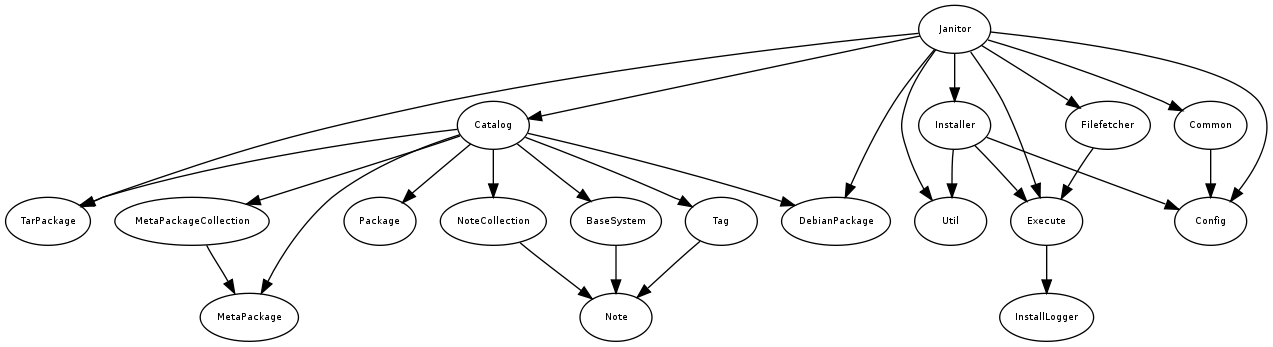
\includegraphics[width=24cm]{images/dependencies.png}
    \mycaption{Modules of the Janitor and their dependencies}{}
 \end{center} 
\vfill
 \label{fig:janitorDependencies} 
\end{figure}
 \end{landscape}

In order to get a more detailed view on the full functionality of the envisioned system it is suggested to consult the 
Design Document\footnote{\href{http://www.knowarc.eu/documents/Knowarc_D1.1-1_07.pdf}
{http://www.knowarc.eu/documents/Knowarc\_D1.1-1\_07.pdf}}.




\section{States of runtime environments}
A major motivation for the managed, manual initiation of dynamic RE
installation is the subsequent manual verification of the installed
packages -- prior to their use in production.
With an automation of the installation, the verification of
that process shall be performed externally to that process.  At this
time, only the automation of the installation has been implemented.
To reflect the progress the external verification has made, REs
are said to be in states. The current implementation lists
installable REs aside the installed REs in the grid information system,
in order to stimulate grid clients to submit packages. The here described
states will be represented to the clients in upcoming developments.

These states are specific for every compute element (CE) and communicated
between the Janitor and the Execution Service. Table~\ref{tab:states} shows all
possible states, while Figure~\ref{fig:RE_states}
displays the transitions between the states that a Runtime Environment may
be in during its life time at a particular CE. \task{?at a particular CE?}  



\begin{table}[!h]
 \begin{center}
 \begin{tabular}{lp{12cm}}
 State&Description\\
 \hline
 UNAVAILABLE&
	The RE is not available for the BaseSystem (see \ref{sec:rdfschema}) the site uses. \\
 INSTALLABLE&
	The RE is available for the BaseSystem the site uses and it
	will be automatically installed once a job requests it. \\
 INSTALLING/a&
	A job requested the RE and it is currently being installed \\
 INSTALLING/m&
	The RE-adminstrator requested the installation of the RE. Its
	currently being installed. \\
 FAILED&
	The installation process failed. \\
 INSTALLED/a&
	The RE is installed dynamically. \\
 INSTALLED/m&
	The RE ist installed manually by the RE-administrator \\
 BROKEN/m&
	The RE is installed but failed tests of the RE-administrator \\
 VALIDATED/m&
	The RE is installed and successfully passed the tests of the
	RE-administrator \\
 REMOVAL PENDING&
	The RE is still installed but will be removed as soon as
	possible. It is not available to new jobs. \\
 REMOVING&
	The RE is currently being removed. \\
 INSTALLED/s&
	The RE was installed in the traditional way by the site administrator. \\
 BROKEN/s&
	The RE was installed in the traditional way and failed
	validation by the RE-administrator, \\
 VALIDATED/s&
	The RE was installed in the traditional way and was
	successfully verified.
 \\
 \end{tabular}
 \end{center}
 \mycaption{States a Runtime Environment can possibly be in.}{}
 \label{tab:states}
 \end{table}

\begin{figure}[!h]
  \begin{center}
    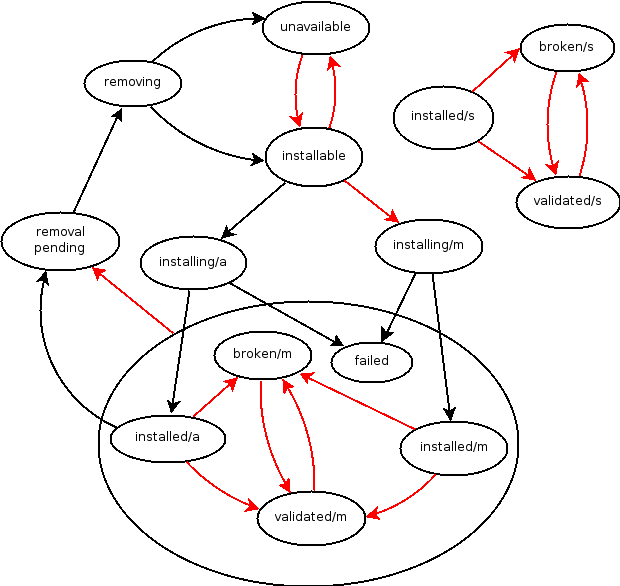
\includegraphics[width=10cm]{images/RE_states.png}
    \mycaption{Relationships between the possible states
 of Runtime Environments.}{Red arcs represent human interaction.
 The distinction between {\bf /a}, {\bf /m} and {\bf /s}
 states does not need to be visible for all clients.}
    \label{fig:RE_states}
  \end{center}
\end{figure}
 
The manually induced transitions are marked in red, he automated transitions in black.
A transition between states can be induced automatically (i.\,e.\ by the
advent of a job requesting a particular dynamic RE) or manually by the
site's supervisor or an individual with respective rights to use the
Janitor's web service.

Upon presentation of a the package name to a Catalog, from which details about
the package are retrieved, a CE may
classify a package to be \texttt{INSTALLABLE} if all the dependencies
are installable or already \texttt{INSTALLED}. The installation can be
performed manually (\texttt{INSTALLING}/{\bf m}) or in an automated fashion
(\ldots/{\bf a}). Should the installation process return an error, then
the installation has \texttt{FAILED}. Once the installation succeeded,
the installed package is validated for its correctness. Should that
process fail, then the package's state it is said to be \texttt{BROKEN}.

Automatically installed packages can be removed by the automatism. A
manually installed package or one that has failed to be installed,
can only be removed upon manual induction.  The \ldots/{\bf s} states
represent those Runtime Environments that are installed in the original
manual way of RE installation in ARC 0.6.

% Runtime Environment are installed for job idenitified by a certain id.


\section{Job states}

The Janitor manages the states that the runtime environments at a particular
compute element are in. However, it is also most important for the Janitor
to be aware of the jobs that depend on the installtion of a RE. REs still in use
should not be removed until the respective job has completed its computations.
The installation or removal of REs by the Janitor is perceived as a mere
consequene of jobs demanding a RE or not, thus, the communcation between
the job-manager AREX and the Janitor will be performed on that 'job level'.

The Janitor has two states for jobs: \texttt{PREPARED} and \texttt{INITIALIZED}. After a job has been succesfully registered 
in the Janitor, its state will be set to \texttt{PREPARED}. Invalid jobs are not cached. 
After the Janitor is requested to deploy the runtime environment, the state of the job will change to \texttt{INITIALIZED}. If 
an unforeseen exception occures during that process, the Janitor will drop the job from its database and set the affected runtime
environments to the state \texttt{FAILED}.

\section{Integration with AREX}


\newenvironment{note}
{\rule{1ex}{1ex}\hspace{\stretch{1}}}
{\hspace{\stretch{1}}\rule{1ex}{1ex}\\}
\begin{note}
The integration into AREX is not completed yet!
\end{note}
\begin{note}
Thus, there will be bigger changes here in this section\dots
\end{note}


\begin{figure}[!h]
  \begin{center}
    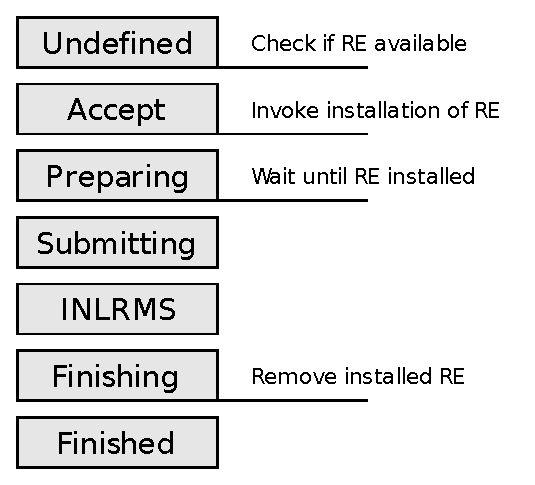
\includegraphics[width=5cm]{images/arex-stages.pdf}
    \mycaption{}{}
    \label{fig:RE_states}
  \end{center}
\end{figure}

\begin{figure}[!h]
  \begin{center}
    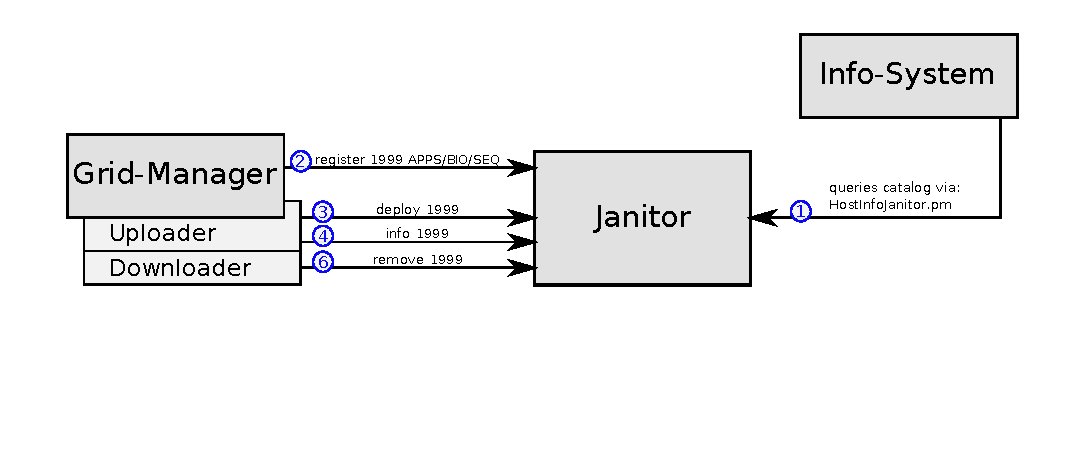
\includegraphics[width=12cm]{images/janitor_integration_2nd_edition.pdf}
    \mycaption{}{}
    \label{fig:RE_states}
  \end{center}
\end{figure}

\section{WebService Interface}

Default port number: 55555\\
Client command equal, except assignment of HED.xml\\
 (from /arc1/trunk:12561)

\begin{figure}[!h]
  \begin{center}
    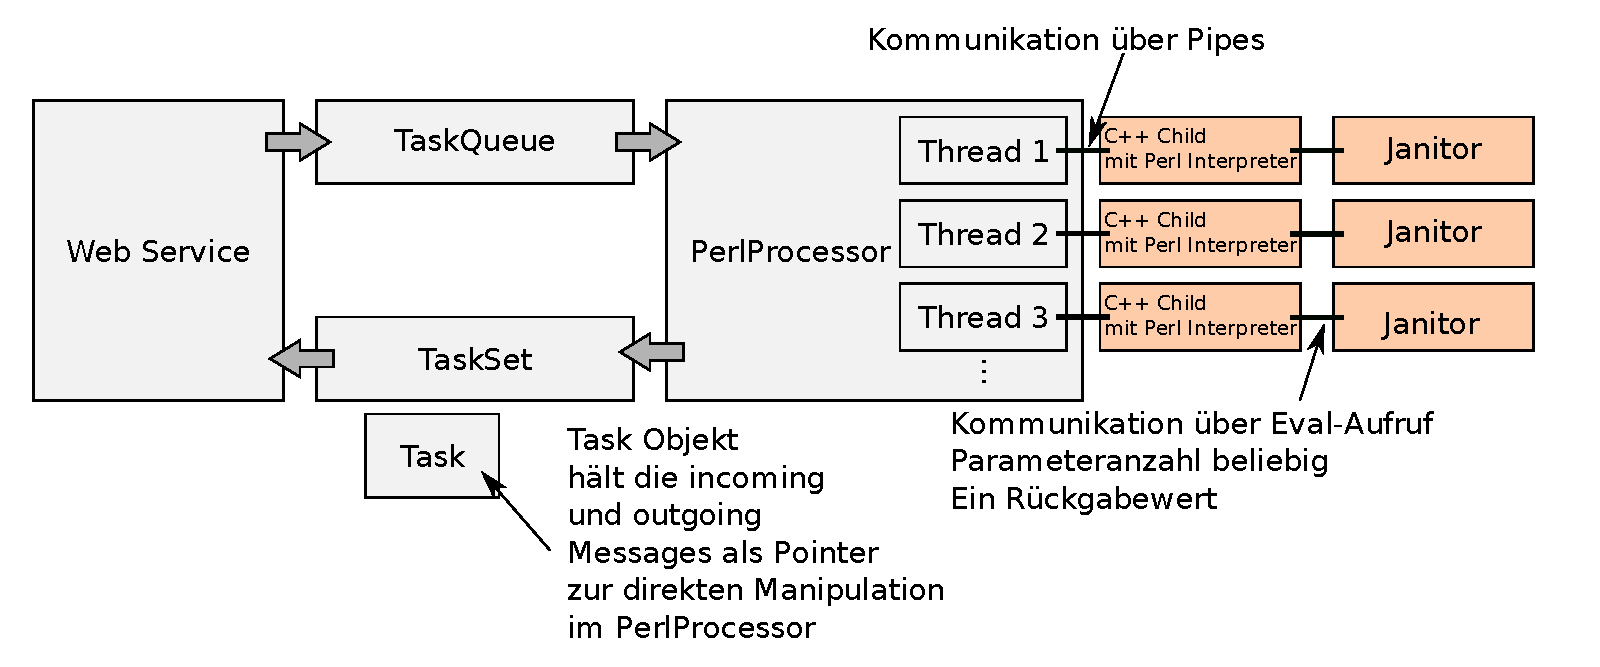
\includegraphics[width=12cm]{images/WS_structure.pdf}
    \mycaption{}{\task{To be translated and beautificated. SVG file is missing!}}
    \label{fig:RE_states}
  \end{center}
\end{figure}

Proposal for SOAP messages:\\
 namespace: dynamicruntime or janitor\\
\task{Create WSDL files for that}
\task{Permission concepts: Depending on certificates. Certain certificates may \texttt{sweep}. Defined in service\_HED.xml. Evaluated in:?? }
\lstsetJUSTXML
\begin{lstlisting}[
        label=lst:SOAPrequest,
        caption={ [Example \textit{arc.conf} settings for janitor.]
                  \textbf{Example \textit{arc.conf} settings for janitor.}}
        ]
<Request action="SEARCH|SWEEP|LIST|DEPLOY|REMOVE|CHECK|REGISTER">
	<Initiator jobid="1234"/>  <!-- Needed for: CHECK|REGISTER|DEPLOY|REMOVE -->
                                  <!-- May contain no jobID in this case a new one will 
                                       be created and returned via the response message-->

	<Runtimeenvironment type="dynamic">      <!-- Needed for: SEARCH|REGISTER-->
		<Package name="APPS/BIO/WEKA-3.4.10"/>
		<Package name="APPS/BIO/WEKA-3.4.11"/>
	</Runtimeenvironment>
                                  <!-- SWEEP and LIST only works, if the TLS-adminstrator identity 
                                       (which is assigned in the arched configuration file) is
                                       to be found by the SecHandler. Both need neither initiator 
                                       nor runtimeenvironment elements -->
</Request>
\end{lstlisting}

\lstsetJUSTXML
\begin{lstlisting}[
        label=lst:SOAPrequest,
        caption={ [Example \textit{arc.conf} settings for janitor.]
                  \textbf{Example \textit{arc.conf} settings for janitor.}}
        ]
<response action="SEARCH|SWEEP|LIST|DEPLOY|REMOVE|CHECK|REGISTER">
	<initiator jobid="1234"/>  <!-- Needed for REMOVE|REGISTER|DEPLOY|CHECK-->
	<result code="0" message="Sucessfully initailized job."> <!-- -->
	<jobs> <!--LIST|CHECK-->
		<job jobid="1234">
			<created>1234567890</created>    <!-- in unix time-->
			<age>0</age>           <!-- in seconds-->
			<runtimeenvironment>
				<package>APPS/BIO/WEKA-3.4.10</package>
			</runtimeenvironment>
			<state>INITIALIZED</state>
		</job>
		<job jobid="4321">
			<created>1234567891</created>
			<age>0</age>
			<package>APPS/BIO/WEKA-3.4.10</package>
			<state>INITIALIZED</state>
			<runtimeenvironmentkey>APPS_BIO_WEKA_3_4_10-835614b62c98c4eb6cb03d74d3161b5d</runtimeenvironmentkey> <!-- at least CHECK -->
			<uses>/nfshome/knowarc/dredesign/src/services/dRE3/perl/spool/runtime/jre__57T1ke1UVz/runtime</uses> <!-- at least CHECK -->
			<uses>/nfshome/knowarc/dredesign/src/services/dRE3/perl/spool/runtime/weka_wHfyytarlE/runtime</uses> <!-- at least CHECK -->
		</job>
	</jobs>

	<runtimeenvironment type="local">      <!-- Needed for: LIST|SEARCH -->
		<package name="APPS/BIO/MUSTANG-3.0-1"/>
		<package name="APPS/BIO/EXONERATE-2.1.0-1"/>
	</runtimeenvironment>

	<runtimeenvironment type="dynamic">      <!-- Needed for: LIST -->
		<package name="APPS/BIO/WEKA-3.4.11">
			<state>INSTALLED_A</state>
			<lastused>1234567890</lastused>
			<jobid>1234</jobid>
		</package>
		<package name="APPS/BIO/WEKA-3.4.10">
			<state>INSTALLED_A</state>
			<lastused>1234567890</lastused>
			<jobid>1234</jobid>
			<jobid>4321</jobid>
		</package>
	</runtimeenvironment>

	<runtimeenvironment type="installable">      <!-- Needed for: LIST -->
		<package name="APPS/GRAPH/POVRAY-3.6">
			<description>The Persistence of Vision Raytracer</description>
			<lastupdate>1234567890</lastupdate>
		</package>
		<package name="APPS/BIO/WEKA-3.4.8A">
			<description>WEKA Machine Learning Software</description>
			<lastupdate>1234567890</lastupdate>
		</package>
	</runtimeenvironment>

</response>
\end{lstlisting}




\section{Janitor file system permissions}

In the current implementation the Janitor perl scripts must be executed as root. In order to execute Janitor with the required permissions,
a setuid wrapper has been prepared. During the installation \task{not done yet} the mode of rjanitor will be set to \texttt{u+s},
i.e. the sticky bit is set to make the binary suid root. \task{According to Daniel: ``A future version of the Janitor will get rid of the suid root helper.''}\\

Thus, Janitor is not executed directly. Instead, a dynamic link will be created in \task{libexec or sbin} which is pointing to
the wrapper.\\

It is suggested to create a user and a group "janitor" for the Janitor.\\

% Currently the Janitor must be executed as root. For this a suid root helper
% is needed. It is provided in /opt/janitor/rjanitor.c. If you installed
% the Janitor in another directory then /opt/janitor change the parameter
% of the execv command in rjanitor.c. Then compile the file with\\
% \texttt{\textdollar gcc -o rjanitor rjanitor.c}\\
% and run as root\\
% \texttt{\textdollar chown root:root rjanitor}\\
% \texttt{\textdollar chmod u+s rjanitor}\\
% to make the binary suid root. A future version of the Janitor will get rid
% of the suid root helper.\\
% 
% The Grid Manager does not call the Janitor directly in /opt/janitor but
% calls /opt/nordugrid/libexec/janitor. So a link is needed (as root):\\
% \texttt{\textdollar ln -s /opt/janitor/rjanitor /opt/nordugrid/libexec/janitor}\\
% \\
% It is suggested to create a user and a group "janitor" for the Janitor.\\
% \\
% The Janitor needs a directory for storing information on installed REs:\\
% \texttt{\textdollar mkdir -p /var/lib/nordugrid/janitor}\\
% \texttt{\textdollar chown janitor:janitor /var/lib/nordugrid/janitor}\\
% \\
% It also needs a directory on the shared volume for installing the REs:\\
% % \texttt{\textdollar mkdir -p $<$shared_volume$>$/janitor}\\
% % \texttt{\textdollar chown janitor:janitor $<$shared_volume$>$/janitor}


\subsection{What happens during installation}

Register
\begin{enumerate}
 \item Look up Catalog and find corresponding runtime environments.
 \item Check if dependcies are available (installed or installable)
 \item Store job in \textit{registrationdir}
\end{enumerate}

Deploy
\begin{enumerate}
 \item Load job out of \textit{registrationdir}
 \item Look up Catalog and find corresponding runtime environments.
 \item Check if dependcies are available (installed or installable)
 \item Download RTEs into the \textit{downloaddir}
 \item $\lbrack$ to be continued or skipped $\rbrack$
\end{enumerate}

\subsection{Security Consideration}



Security is a major concern for grid systems. Any additional feature
and especially an automatic software
installation inheritently introduces security threats. This section
addresses those and describes the available solutions to limit
security risks.

In the current installation, every user authorised to execute a job is
also authorised to install a REs. Restrictions are
only imposed on the set of dynamic REs that are available for installation.
Restrictions are imposed by the site admininistrators on the descriptions
that are given by the Catalog that is offering the package. These
descriptions may explicitly mention dynamic REs' names, e.g. a regular expression on
these, or refer to tags of packages that categorise these. However,
the core of these controls lies with the maintainers of the Catalog,
who needs to be trusted.

All dynamic REs are installed in separate directories. The provisioning of
disk space is the duty of the site administrator.  In the current
implementation, the installation is completely transparent to the user:

\begin{itemize}
\item Dynamic REs are not distinguished between {\em installed} and
  {\em installable} in the information system.
\item No status information is given at the time a dynamic RE is installed.
\end{itemize}

Malevolent regular users with respective training in using system exploits
to gain root access are likely to find security holes by regularly
submitted scripts.  The authentication and authentification of users,
together with respective logging, is the major defense against such
attacks. What is consequently left to be protected against are unwanted
side-effects by the installation of software.

The worst case scenario would be the installation of a RE
that overwrites system files. With the current implementation, which is
based solely on tar files, this is barely possible, unless such is
performed by the install scripts that accompany the tar files. However,
hereto the installation would have to be performed by a user with system
priviledges, for which there is no technical requirement.

The installation of packages from the Debian distribution (or other
packages of mainstream Linux distributions) is seeked to reduce the
complexity and burden in the maintenance for dynamic REs. In the
current implementation, Debian packages may be installed only by their
transformation into tar files. With the advent of the interface for
the virtualisation of the grid infrastructure, it is anticipated to
work with native packages of the Debian Linux distribution. The reuse
of packages that passed many eyeballs - as it is the case with packages
from major Linux distribution - security is further increased or becomes
as high as with the operating system underneath virtual clients.

Summarising, there is general concern about the security of grid
computing.  Dynamic REs introduce new dangers since a
manual control at the grid site is substituted by a remote process that
is out the direct supervision of a local site administrator. The signing
of packages by known and directly or indirectly trusted developers is
a good indicator that no malevolent individuals have tampered with the
binary. The site administrators can limit the sources of packages and
specify packages that are eligible or excluded from installations.



% * Programming concept
% ** design decisions: Perl, RDF, Two classes entities with states: jobs and rtes
% ** State transitions of RTEs
% ** State transitions of Jobs
% ** RDF based knowledge base for runtime environments
% ** File based recovery of Jobs and RTEs
% ** Class structure
% ** Interaction with A-REX
% 
% 5
\chapter{Outlook}
% 
% * Future work
% ** API and WebService-Interface for Janitor
% ** Glue2 specification for RTE states
% 

\section{Representation of dynamic REs in the information model}
Dynamic REs require an extended representation in the
information model.  The Application Software description should be able
to distinguish installed REs from installable REs, potentially offer
descriptions of extended RE state-like information. This work is planned
to be carried out as part of the Glue-2.0 effort of OGF\footnote{OGF
GLUE: https://forge.gridforum.org/sf/projects/glue-wg}.

\section{Integration with Workflow Management}

Future development of ARC aims at integrating grid computing with
workflow tools for the web services that have a growing user base in
bioinformatics. The challenge is to prepare REs for
programs or databases and to offer such concisely to users of the
workflow environments.  In the bioinformatics community, such are
today offered as web services.  This anticipated development instead
fosters the dynamic installation on the grid whenever appropriate to
allow for special computational demands in high-throughput analyses.
Conversely, because of the increased complexity of workflows with respect
to the already today not manually manageable number of REs, without an
automatism for the automated installation of software packages on the
grid, the use of workflows in grid computing seems mute.

\section{Implementation of a Catalog service}
 
A Catalog service is planed to be implemented on top of the ARC
HED component.  This service will render the currently used locally
accessible RDF file externally accessible. Selected users are then allowed
to remotely add/edit/remove REs to/from to it.  The Janitor will access
the content of the Catalog through a well-defined Web Service interface.

\section{Integration with the Virtualization work}

The RDF schema nicely prepares for the upcoming virtualisation of worker
nodes.  How exactly the dynamics are integrated will depend on how
dynamic the virtualisation of the nodes is. In the simplest scenario,
a worker node's CPU will only be occupied by a single virtual machine
and that will not be changed. In this case, there is no difference to
the setup of the Janitor with today's static setups.

However, if the BaseSystems can be substituted dynamically, then a RE
can possibly be offered via multiple BaseSystems. The RDF
Schema describes BaseSystems as separate instances and as such differs
from the current RE registry.  Heuristics that prefer one BaseSystem for
another can make direct use of the data that is presented in the schema.
The integration of packages from Linux distributions in the description
of REs is essential to have a means to decide for the equivalence of
manual additions and the functionality that comes with BaseSystem.

\section{Use of RDF}

The RDF is "correctly" used within the Janitor via the Redland libraries.
What is still missing is a semantical reasoning on what packages to
allow or disallow. For instance: allow all packages associated with
bioinformatics. This shall wait a bit longer until more experiences
on the community's demand for this service have been made.

\section{Manual Verification}

There is yet no explicit notion of a concept on how users can report
on the reliability of individual compute nodes and use such information
for the decision making on where to sent their jobs. And with an increasing
complexity of software installed, being used across versions, one will
rather trust one's very own experiences for individual sites than some
external repository or other pieces of information that may be weeks
or months old.

Consequently, no means for a manual verification and the communication
of results of such have yet been implemented.


\section{Known issues}
\begin{itemize}
 \item There is a arc.conf file in which all possiblie flags are listed... ADD THE JANITOR FLAGS!!!
 \item Dynamic RTEs are now listed as manually installed in the ``janitor list'' command.. change that
\end{itemize}
% 6
\chapter{Appendix}

\section{Useful tutorials and documentations}

In order to learn more about ARC several other tutorials and documentations have been written:
\begin{itemize}
 \item ARC Web Services Quick Usage Guide~\cite{2008_UNKNOWN}
 \item The Hosting Environment of the Advanced Resource Connector middleware~\cite{2008_Cameron}.
 \item Security framework of ARC1~\cite{QIANG_2008}.
 \item Documentation of the ARC storage system~\cite{Nagy_2008}.
 \item Eclipse WTP 1.5.1, Introduction to the WSDL Editor, \url{http://wiki.eclipse.org/index.php/Introduction_to_the_WSDL_Editor}


\end{itemize}




\section{Important XSD files}\label{sec:impXSD}

\lstsetJUSTXML
\lstinputlisting
	[
	label=lst:mcc.xsd,
	caption={[XML schema of configuration files.]\textbf{XML schema of configuration files.}}
	]{../../../src/hed/libs/loader/mcc.xsd}

\lstsetJUSTXML
\lstinputlisting
	[
	label=lst:tcp.xsd,
	caption={[XML schema of the TCP component.]\textbf{XML schema of the TCP component.}}
	]{../../../src/hed/mcc/tcp/tcp.xsd}

\lstsetJUSTXML
\lstinputlisting
	[
	label=lst:tls.xssd,
	caption={[XML schema of the TLS component.]\textbf{XML schema of  the TLS component.}}
	]{../../../src/hed/mcc/tls/tls.xsd}

\lstsetJUSTXML
\lstinputlisting
	[
	label=lst:http_xsd,
	caption={[XML schema of the HTTP component.]\textbf{XML schema of the HTTP component.}}
	]{../../../src/hed/mcc/http/http.xsd}









% 
% Questions:
% \begin{itemize}
%  \item The images of the HED structure always are ordered like: TCP - TLS - HTTP - PLEXER - SOAP - Web Service   but the source code examples are: TCP - TLS - HTTP - SOAP - PLEXER - Web Service\\
% --- ANSWER BY WEIZHONG: In my understanding (because plexer is not my initial idea), plexer (as a sort of hub) can be put at both after http or soap. If you put after soap,then you are doing switching for different web services. While I put it after http, because somehow, I need to switch the message after http-processing, in more detail, one branch for soap and then web service/s,
%  one branch for a non-soap service/server (the SP Service is not a service based on SOAP, actually it is based on http, so it is kind of web application).
% 
% \item The HED does not act as a front end server which delegates its task to new instances acting on a diffrent port such that the daemon is always available. 
% \end{itemize}

% 
% 
 \task{RENAMING HED configuration file into~ARC service configuration file - proposed by Marek}
 \task{(echo service) client configuration file - proposed by Marek}
 \task{Check commas using \url{http://leo.stcloudstate.edu/punct/comma.html}}

 \task{Bisher noch nicht beachtet: \\
\\\textcolor{urgent}{
In general, a comma is used when the
subordinate clause precedes the main clause, like this:\\
\\
``When subjects were aware of the purpose of the experiment, no effect was
observed.''\\
\\
Furthermore:\\
\\
      ``We discarded specimens that had become contaminated.''\\
\\
In this case, the relative clause is restrictive because it defines exactly which specimens
were discarded. Restrictive clauses should not be preceded by a comma.\\
\\
  In contrast, a non-restrictive clause gives additional information about an object that
has already been identified; for example:\\
\\
      ``The file server uses the XFS file system, which supports journaling and pro-
      vides excellent performance.''\\
\\
In this case, the relative clause does not restrict or define the particular file system being
talked about, but merely provides additional information. Non-restrictive clauses should
be preceded by a comma.}}



% 7

 \bibliography{literature}
 \bibliographystyle{IEEEtran}                       % A nice bibliography style


\end{document}
